%%%%%%%%%%%%%%%%%%%%%%%%%%%%%%%%%%%%%%%%
%% MCM/ICM LaTeX Template %%
%% 2023 MCM/ICM           %%
%%%%%%%%%%%%%%%%%%%%%%%%%%%%%%%%%%%%%%%%
\documentclass[12pt]{article}
\usepackage{geometry}
\geometry{left=1in,right=0.75in,top=1in,bottom=1in}

%%%%%%%%%%%%%%%%%%%%%%%%%%%%%%%%%%%%%%%%
% Replace ABCDEF in the next line with your chosen problem
% and replace 1111111 with your Team Control Number
\newcommand{\Problem}{C}
\newcommand{\Team}{2319197}
%%%%%%%%%%%%%%%%%%%%%%%%%%%%%%%%%%%%%%%%

\usepackage{newtxtext}
\usepackage{amsmath,amssymb,amsthm}
\usepackage{newtxmath} % must come after amsXXX
\usepackage{indentfirst}
\usepackage{multirow}
\usepackage{lipsum}
\usepackage{caption}
\usepackage{subfigure}
\usepackage{url}
\usepackage{siunitx}


\usepackage[pdftex]{graphicx}
\usepackage{xcolor}
\usepackage{fancyhdr}
\usepackage{pdfpages}
\lhead{Team \Team}
\rhead{}
\cfoot{}
\title{A Data Analysis and Prediction Model Based on Supervised Learning and Clustering Algorithm}

\newtheorem{theorem}{Theorem}
\newtheorem{corollary}[theorem]{Corollary}
\newtheorem{lemma}[theorem]{Lemma}
\newtheorem{definition}{Definition}
\renewcommand{\arraystretch}{1.4}

%%%%%%%%%%%%%%%%%%%%%%%%%%%%%%%%
\begin{document}
\graphicspath{{.}}  % Place your graphic files in the same directory as your main document
\DeclareGraphicsExtensions{.pdf, .jpg, .tif, .png}
\thispagestyle{empty}
\vspace*{-16ex}
\centerline{\begin{tabular}{*3{c}}
	\parbox[t]{0.3\linewidth}{\begin{center}\textbf{Problem Chosen}\\ \Large \textcolor{black}{\Problem}\end{center}}
	& \parbox[t]{0.3\linewidth}{\begin{center}\textbf{2023\\ MCM/ICM\\ Summary Sheet}\end{center}}
	& \parbox[t]{0.3\linewidth}{\begin{center}\textbf{Team Control Number}\\ \Large \textcolor{black}{\Team}\end{center}}	\\
	\hline
\end{tabular}}
%%%%%%%%%%% Begin Summary %%%%%%%%%%%
% Enter your summary here replacing the (red) text
% Replace the text from here ...
\begin{center}
\textbf{Summary}
\end{center}

\indent With the emergence of various puzzle games, people can spend their fragmentation time with fun and joy. At the same time, maintainers of these games may natually wonder the present and future situation of the game. The editor of \textbf{Wordle}, one of those popular games, is eager to know the analysis of past data and the future prediction. In view of this, we modeled the variation of the \textbf{number of reported results} of Wordle found on Twitter and the \textbf{distribution} of it, as well as the \textbf{classification} of words by difficulty to reach the goal.

Several models are established Model I: Multilayer Perceptron; Model II: Gradient Boosting Decision Tree and Multilayer Perceptron; Model III: K-Means and K-Nearest Neighbour, etc.

Before all the models are established, we delete all the wrong data in order to do better analysis. Moreover, we conduct a wide range of correlation tests and \textbf{visualize} them so as to make results more intuitive.

For Model I: Based on the \textbf{heat map} about the correlation of raw data, we found that the appearing frequency of the word 'Wordle' as well as the daily word are related to the number of reported results and percentage of hard mode results. Considering that there are multiple inputs to the model, we build \textbf{Multilayer Perceptron} to fit curves and make predictions on March 1, 2023. We use prediction of the number of reported results and the scaling of prediction of hard mode results as two boundary of interval. The results are shown in Table 1.

For Model II: This model is actually an extension of Model I. The difference lies in the participation of \textbf{Gradient Boosting Decision Tree} for improvement. Due to the fact that there exists a strong correlation between Tries, we choose the better output of the two models and use it as as the input for the next prediction. It can be concluded that through the number of repeated letters in words, the frequency of word appearing on Google and Twitter and Tries can we make predictions on the distribution of reported results, it will be shown in Table 2.

For Model III: To tackle the problem of classifying the words by difficulty, \textbf{K-Means} and \textbf{K-Nearest Neighbour} are good choices. Using K-means can seperate data into clusters and K-Nearest Neighbour is capable of categorizing words into clusters. We set up five clusters as five levels of difficulty and the result for word EERIE is shown below Table 3.

Finally, we conduct sensitivity analysis on our model, in which our model performs a nearly 5\% fluctuation when we take data with outliers as input, showing that our model can be applied to different times. Meanwhile, we use \textbf{Python Web Crawler} that can automaticlly fetch data from \textbf{Google Books} for future extensions. The model can be considered stable. Afterwards, a letter with our results are sent to \textit{New York Times} Puzzle Editor.

\vspace{1cm}
\noindent\textbf{Keywords:} Wordle; Data Analysis and Prediction; Multilayer Perceptron; Gradient Boosting Decision Tree; K-means; K-Nearest Neighbour; Web Crawler; Sensitivity Analysis
% to here
%%%%%%%%%%% End Summary %%%%%%%%%%%

%%%%%%%%%%%%%%%%%%%%%%%%%%%%%%
\clearpage
\pagestyle{fancy}
% Uncomment the next line to generate a Table of Contents
%\tableofcontents 
\newpage
\setcounter{page}{1}
\rhead{Page \thepage\ }
%%%%%%%%%%%%%%%%%%%%%%%%%%%%%%
\maketitle
\tableofcontents
\newpage

\section{Introduction}
\subsection{Problem Background}
\indent Online little puzzle games are more and more popular in these times due to their lightness and fun. Among those that had aroused a vast trend, Wordle, which is a word puzzle offered by \textbf{\textit{New York Times}}, is definitely worth mentioning. 

In the game, a guess of a word that equals to the answer can leads to the success of the game and players only have at most six trials before they lose the game. Two modes are provided in the game, normal mode and hard mode. The hard mode of Wordle makes the game more tricky, because once the player finds the correct letters in a word, which will be clued by the color of tiles, these letters must be used in the subsequent guess.

For \textbf{\textit{New York Times}} puzzle editor, the estimated future data like the number of total trials or the distribution of reported results may be helpful to him to make decisions on advertising or further improving the game. So the question lies in predicting these features as percise as possible using mathematical modeling.

\subsection{Restatement of the Problem}
Considering the background information and restricted conditions identified in the problem statements, we need to solve the following problems :

$\bullet$ \textbf{Problem 1} 

We need to build a model and analyze the trend, and use our model to generate a prediction interval on March 1, 2023. After that, we should determine the attributes of the word that may affect the report percentage in Hard Mode.

$\bullet$ \textbf{Problem 2} 

Build a model to predict trial distribution, then analyze its feasibility and uncertainties on word \textbf{\textit{eerie}} on date March 1, 2023

$\bullet$ \textbf{Problem 3} 

Develop a model to classify words by it's difficulty and analyze its attributes which are associated with clusters, then apply it to word \textbf{\textit{eerie}} and compute accuracy.

$\bullet$ \textbf{Problem 4} 

Demonstrate some intersting features of data set.

\newpage
\subsection{Our Work}

\begin{figure}[htbp]
	\centering
	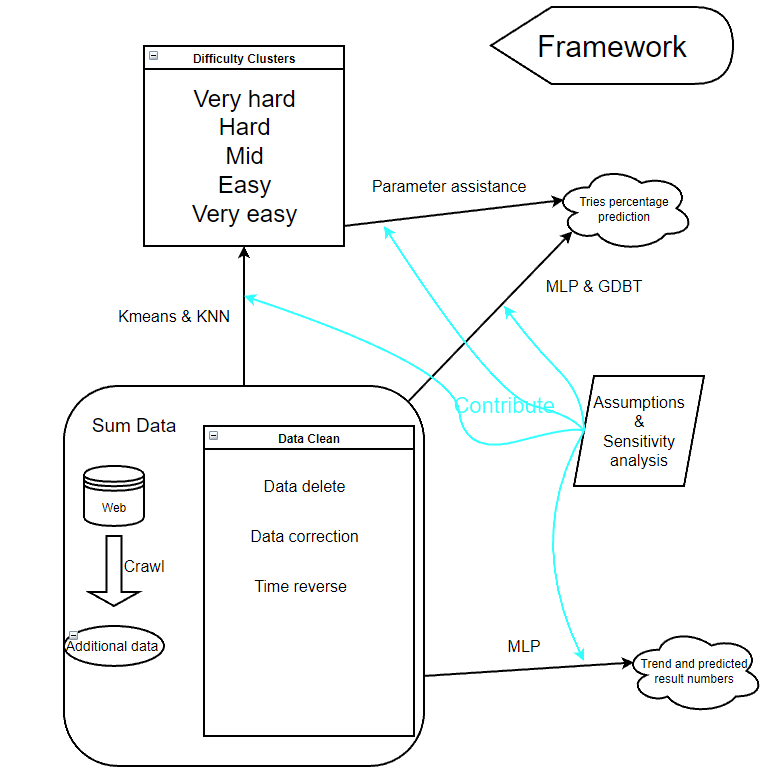
\includegraphics[height=12cm, width=12cm]{our_work.png}
	\caption{\textit{A mind map of our whole work}}
	\end{figure}

	By analyzing and cleaning provided data and crawling some additional word data from some websites, we first get the sum manipulated data set. Next we find and modify some models to handle different problems with contributory assumptions and sensitivity analysis. After get word difficulty clusters classification, we use it as auxiliary with primary MLP,GDBT model to resolve trend,result numbers,tries percentage prediction.




\section{Assumptions and Justification}
$\bullet$ \textbf{Assumption 1} 

The popularity of game Wordle is associated with searching frequency of the word 'Wordle'.

$\hookrightarrow$ \textbf{Justification}

We use Python Web Crawler to obtain the number of reports and advertisement on Wordle from  Google Books. The data shows that after April,2022, reports on Wordle was reduced to a very limited number.

$\bullet$ \textbf{Assumption 2} 

We believe that different results of trials are dependent to each other.

$\hookrightarrow$ \textbf{Justification} 

We run a correlation test and Pearson P-value test on this. The result is on \textbf{Figure 2, 3}.

$\bullet$ \textbf{Assumption 3}

We believe that replacement from date to numbers is valid.

$\hookrightarrow$ \textbf{Justification} 

Since the global festival factor can't be unified, the increase of dates is the same as the increase of continous integer numbers.

\textbf{All other tests on correlation coefficient and P-value of Pearson correlations will be shown on 4.1, 5.1 or 6.1. We use the commonly acknowledged standard P-value of 0.05 as our criterion of acceptable.}

\begin{figure}[htbp]

	\centering
	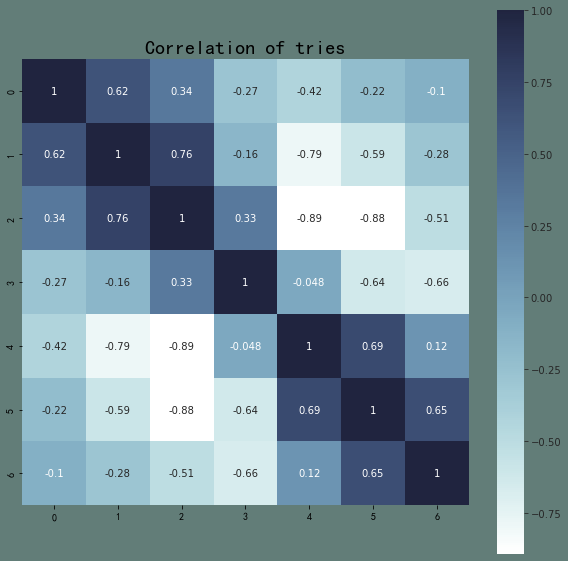
\includegraphics[height=10cm, width=10cm]{tries_cor.png}
	\caption{Correlations between tries, 0-6 respectively represent 1 tries to X tries}


\end{figure}

\begin{figure}
	
\centering
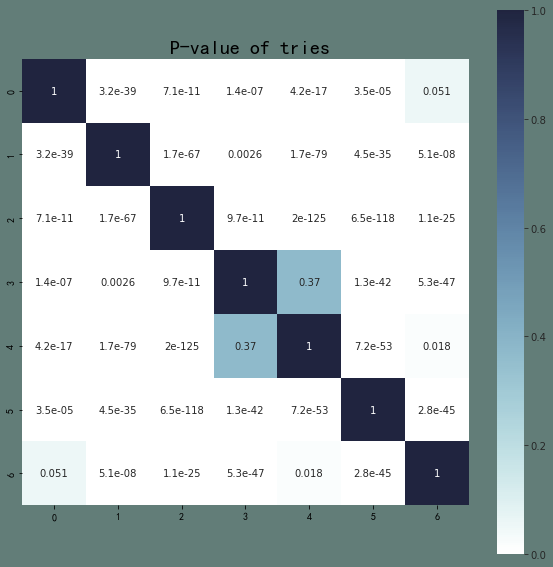
\includegraphics[height=10cm, width=10cm]{per_tries.png}
\caption{Correlations between tries, 0-6 respectively represent 1 tries to X tries}
\end{figure}

\section{Model I : Multilayer Perceptron}
\subsection{Data Description}

In the data preprocessing stage, we analyze the data of reported result and hard mode, finding that the curves of these two factors are highly relevant. We also curve the search frequency of \textbf{Wordle} on the data obtained from Web Crawler in which the frequency are regarded as the popularity of the game. Comparing these curves, we suprisingly notice that the curve of search frequency of \textbf{Wordle} is highly identical to the previous two curves. Graphs of three curves will be demonstrated in \textbf{Figure 4}.

For the identical feature of reported result and hard mode, we introduce a new feature called \textbf{"Zoom Ratio"}. Zoom Ratio is calculated through
\begin{equation*}
	Z = \frac{X_{reported\ result}}{Y_{hard\ mode}}
\end{equation*}
where Z denotes Zoom Ratio, X and Y are respectively reported results and hard mode.

We encode the date to number and normalize all the model input and output using the equation,
\begin{equation*}
	X_i = \frac{X_i - X_{mean}}{Standard\ Deviation}
\end{equation*}
where $X_i$ denotes the normalized data, $X_{mean}$ denotes the mean of input sequence.

We also compute the Pearson coefficient and its P-value of reported result, hard mode, zoom ratio, search frequency of \textbf{Wordle} and appearing frequency of each word. Results are shown in \textbf{Figure5,6}.

The remnant results are shown in appendix.


% \begin{figure}[htbp]
% 	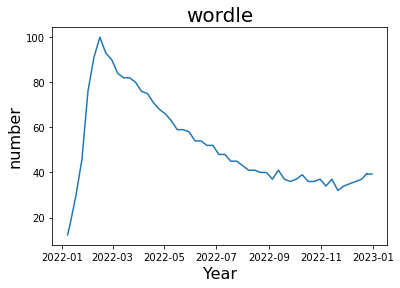
\includegraphics[height=10cm, width=10cm]{wordle.png}
% 	\caption{The cureve of wordle}
% 	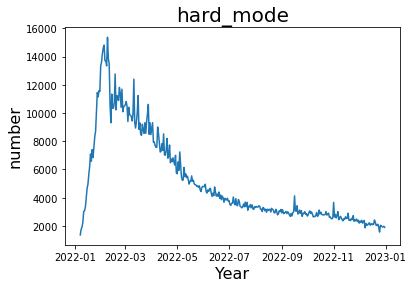
\includegraphics[height=10cm, width=10cm]{hard_model.png}
% 	\caption{The cureve of hard mode}
% 	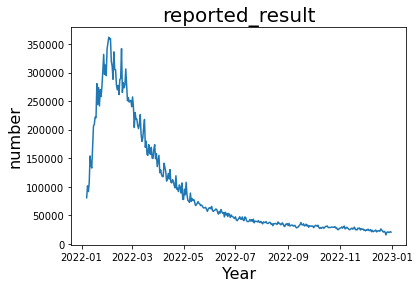
\includegraphics[height=10cm, width=10cm]{reported_result.png}
% 	\caption{The cureve of reported result}

% \end{figure}



\subsection{Overview of the Model}
A multilayer perceptron (MLP) is a fully connected class of feedforward artificial neural network (ANN). The term MLP is used ambiguously, sometimes loosely to mean any feedforward ANN, sometimes strictly to refer to networks composed of multiple layers of perceptrons (with threshold activation). Multilayer perceptrons are sometimes colloquially referred to as "vanilla" neural networks, especially when they have a single hidden layer.

\subsection{The Establishment of Model I}
We have three candidate models due to the following reasons:

\textbf{Multilayer Perceptron}: Hereinafter referred to as "MLP", is a many-to-one machine learning model. Considering that we have multi-input such as date, search frequency of \textbf{Wordle} and the number of repeated letters, MLP is a reasonable choice.

\textbf{Gray Prediction}: Due to the influence of date, we should take Time Series Model into consideration, in which case Gray Prediction is a proper choice with following prediction equation,
\begin{equation*}
	\hat{x}^1(k+1) = [x^0(1)-\frac{b}{a}]e^{-ak} + \frac{b}{a}
\end{equation*}
where a, b are the coefficients and ${x^1(1),x^1(2),...,x^1(n)}$ are the result of 
\begin{equation*}
	x^m(k) = \sum_{i=1}^{k}X^{m-1}(i)
\end{equation*}
as ${x^0(1),x^0(2),...,x^0(n)}$ is the original sequence.

\textbf{Polynomial Prediction}: We notice that on the right half of the curve on report results, the line is smooth and monotonically decreasing, so we choose polynomial prediction according to equation,
\begin{equation*}
	y(x,w) = w_0 + w_1x + w_2x^2 + ... + w_mx^m = \sum_{j=1}^{m}w_jx^j
\end{equation*}
where $w_m$ denotes the coefficients of the polynomial.
\subsection{The Solution of Model I and Question I}
We choose different inputs inorder to fit different models. The Root Mean Squared Error, hereinafter referred to as "RMSE", of the three models are listed below.
\vspace{0.2cm}
\begin{center}
\begin{tabular}{c c c c}
\hline
value & MLP & Polynomial prediction & Grey Prediction\\
\hline
$RMSE(reported\ result)$&0.16995&0.33027&0.41211\\
$RMSE(hard\ mode)$&0.34914&0.52607&0.56249\\
$RMSE(zoom\ ratio)$&0.13120&0.37287&0.47575\\
\hline
$Output(reported\ result)$&20490&15097&6365\\
$Output(hard\ mode)$&1911&1655&1380\\
$Output(zoom\ ratio)$&9.655&10.285&4.534\\
\hline
\end{tabular}
\vspace{0.2cm}
\end{center}

\textit{Table 1: RMSEs and Output(Prediction) of reported results, hard mode and percentage of them.}
\vspace{0.5cm}

Comparing with Polynomial Prediction and Grey Prediction, MLP has a much better performance on three RMSEs and thus we choose \textbf{MLP} to be the solution model for Question I.


In order to predict an interval for the number of reported results on March 1, 2023, we use the prediction of reported results as one boundary, the product of the prediction of hard mode and the prediction of zoom ratio as another to generate the prediction interval.

The predicted result of the interval for reported result on March 1, 2023 is \textbf{[18450, 20490]}. As for the attributes of the word, we take a Pearson Correlation Test on the number of repeated letters, the number of vowels, and the frequency of word appearing on Google Books, finding that the percentage of players reported to play in Hard Mode is related to the frequency of the word with a P-value of 0.006, which is less than 0.05 and thus highly acceptable. Results are shown in  \textbf{Figure7,8}.

\subsection{The Solution of Question IV}
There are some words that are misspelling, such as ‘clean’ is written to ‘clen’ and ‘probe’ is written to ‘rprobe’. Besides, there exists a word ‘naïve’ in which ‘ï’ is unrecognizable by some algorithms. So we delete the wrong words and ‘naïve’. 

Another interesting point lies in the fact that the percentage of Tries 7 decreases as time goes. If we compute an average value of Tries 7 every 7 rows, we can find that as time flies, people are more unlikely to end the game in 7 or more times.


\begin{figure}[htbp]
	\centering
	\subfigure[]{
	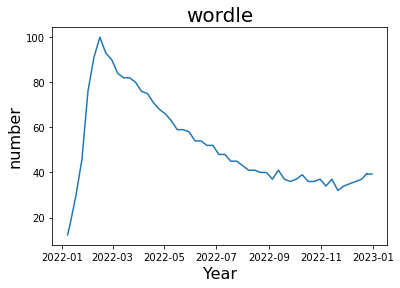
\includegraphics[width=8.5cm,height=5cm]{wordle.png} \label{Fig.4(a)}
}
	\hspace{2mm}
	\subfigure[]{
	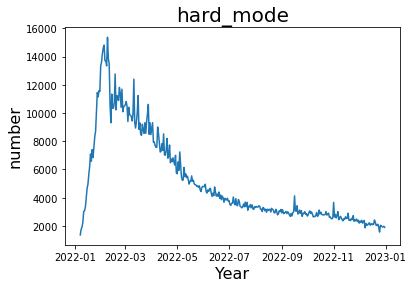
\includegraphics[width=8.5cm,height=5cm]{hard_model.png} \label{Fig.4(b)}
}	
	\hspace{2mm}
	\subfigure[]{
		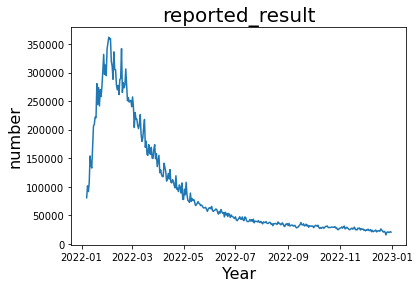
\includegraphics[width=8.5cm,height=5cm]{reported_result.png} \label{Fig.4(c)}
	}
	\hspace{2mm}
	\subfigure[]{
		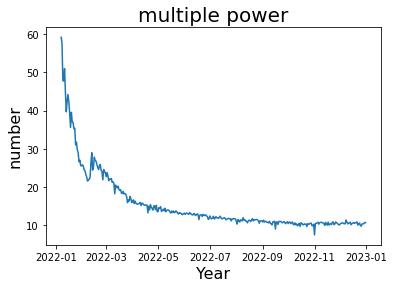
\includegraphics[width=8.5cm,height=5cm]{mul.png} \label{Fig.4(d)}
	}
	\caption{Four original curves of data.}
\end {figure}

\begin{figure}
	
	\centering
	
	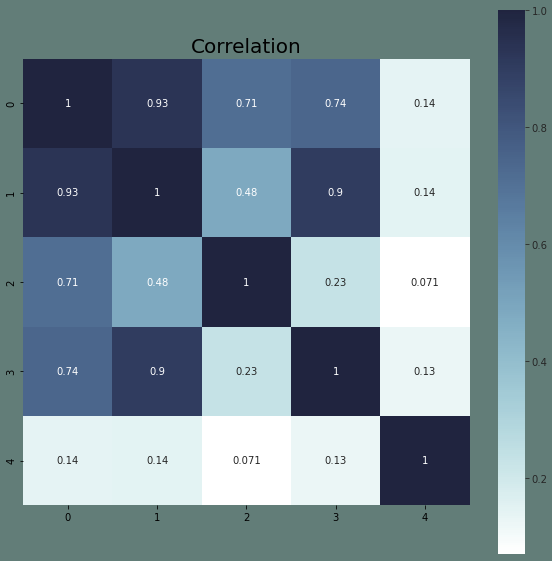
\includegraphics[height=9cm, width=9cm]{COR_re.png}
	\caption{Correlations, 0:reported result,1: hard mode,2:Zoom ratio,3:the frequency of wordle,4:the frequency of words}
	\end{figure}
	
	\begin{figure}[htbp]
	
		\centering
		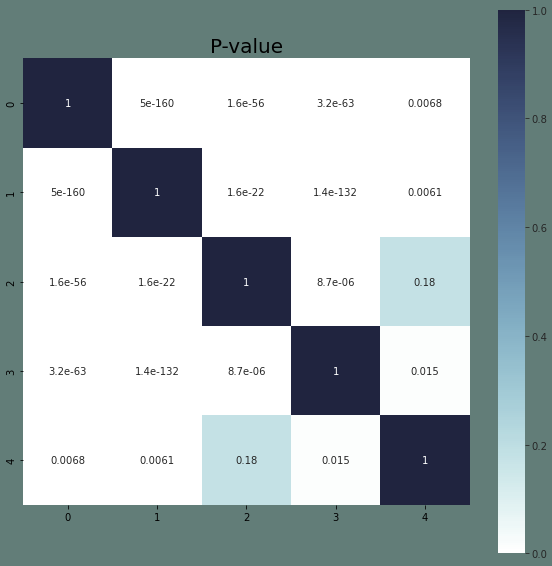
\includegraphics[height=9cm, width=9cm]{PER_re.png}
		\caption{P-value,0:reported result,1: hard mode,2:Zoom ratio,3:the frequency of wordle,4:the frequency of words}
	
\end{figure}

\begin{figure}
	
	\centering
	
	\includegraphics[height=9cm, width=9cm]{COR_m1_re.png}
	\caption{Correlations, 0:Zoom ratio,1:hard mode,2: the number of repeated letters,3:the number of vowels,4:the frequency of words}
	\end{figure}
	
\begin{figure}[htbp]
	
		\centering
		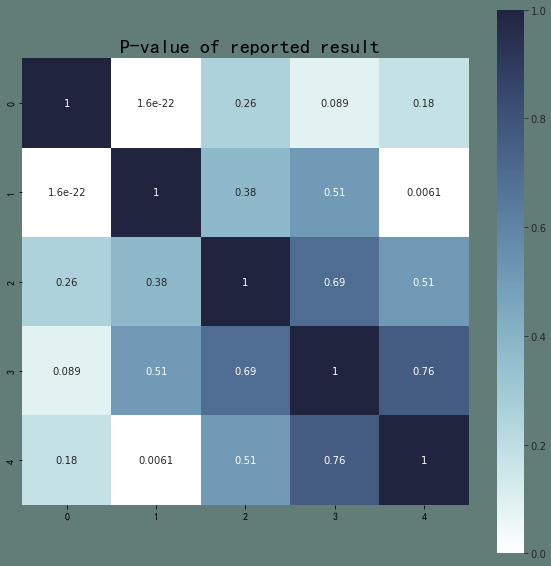
\includegraphics[height=9cm, width=9cm]{Per_m1_re.png}
		\caption{P-value,0:Zoom ratio,1:hard mode,2: the number of repeated letters,3:the number of vowels,4:the frequency of words}
	
\end{figure}
\newpage{}
\section{Model II : MLP and GBDT}
\subsection{Data Description}
We have defined a new equation based on tries to define the difficulty level of a word. The equation is as follows,
\begin{equation*}
	difficulty\_score = \sum_{i=1}^{7}2^{i}*x_{tries}
\end{equation*}
where $x_{tries}$ denotes the percentage of attempt times in the raw data. 
We encode the date to number and normalize all the model input and output using the equation same to model1.
We compute the Pearson coefficient and its P-value of the obtained difficulty level and all the previously obtained information.We also conducted a correlation analysis and p-value test on the tries, and the results we obtained are \textbf{Figure9,10,11}.

The remnant results are shown in appendix.

\subsection{Overview of the Model}
Gradient boosting is a machine learning technique used in regression and classification tasks, among others. It gives a prediction model in the form of an ensemble of weak prediction models, which are typically decision trees. A gradient-boosted trees model is built in a stage-wise fashion as in other boosting methods, but it generalizes the other methods by allowing optimization of an arbitrary differentiable loss function.
\subsection{The Establishment of Model II}
Due to the fact that the samples still have multiple dimensions, a machine model can be a good choice.We choose the following two models owing to these reasons.

\textbf{MLP}: We choose MLP for the similiar reason in model I.

\textbf{Gradient Boosting Decision Tree}: Hereinafter referred to as ”GBDT”, is a type of machine learning algorithm that combines multiple decision trees to make predictions, which fullfills our need to use many-to-one models. Comparing to other machine learning models, GBDT performs the best RMSEs. For GBDT, we use \textbf{GridSearchCV} to find the best parameters.

\subsection{The Solution of Model II and Question II}
Through correlation analysis, it was found that the number of repeated letters and frequency of occurrence of a word are closely related to the difficulty level of a word.Therefore,We have decided to use the number of repeated letters and word frequency to predict tries.There is also a intimate correlation between different tries.Therefore, we improved the original model by \textbf{using the better output of the two models and use it as as the input for the next prediction}, turning it into a memory model. AS the following equation:
\begin{equation*}
	X_{i+1} = \alpha_i Output_{i}|_{RMSE\_lower\_model} + \beta_i
\end{equation*}
where $X_{i+1}$ is the input of Tries $i+1$ model, $ \alpha_i$ is the coefficient, $Output_{i}$ is the output of the Tries i model and $\beta_i$ is a constant.
Since each model has its own strengths, we have chosen to use a hybrid model.the results we obtained are as follows.
\vspace{0.2cm}
\begin{center}
\begin{tabular}{c c c c c c c c}
\hline
value & Tries 1 & Tries 2 & Tries 3 & Tries 4& Tries 5& Tries 6& Tries X \\
\hline
$RMSE(GBDT)$&1.3305&0.8397&0.8781&0.9937&0.2922&0.3500&0.8104\\
$RMSE(MLP)$&1.0785&1.1645&0.9527&0.8522&0.5017&0.2053&0.4949\\
\hline
$Output(GBDT)$&0\%&1.83\%&34.86\%&29.35\%&11.92\%&5.50\%&16.51\%\\
$Output(MLP)$&0\%&6.74\%&31.46\%&37.07\%&16.85\%&6.74\%&1.12\%\\
\hline
$Mixed\ Result$&0\%&2.15\%&40.86\%&35.48\%&13.97\%&6.45\%&1.07\%\\
\hline
\end{tabular}
\vspace{0.2cm}

\textit{Table 2: RMSEs and Output(Prediction) of GBDT and MLP.}

\textit{'Tries X' infers to Tries that are more than 7(including 7).}

\textit{'Mixed Result' in the table is our prediction for Question II.}
\end{center}

\begin{figure}
	
	\centering
	
	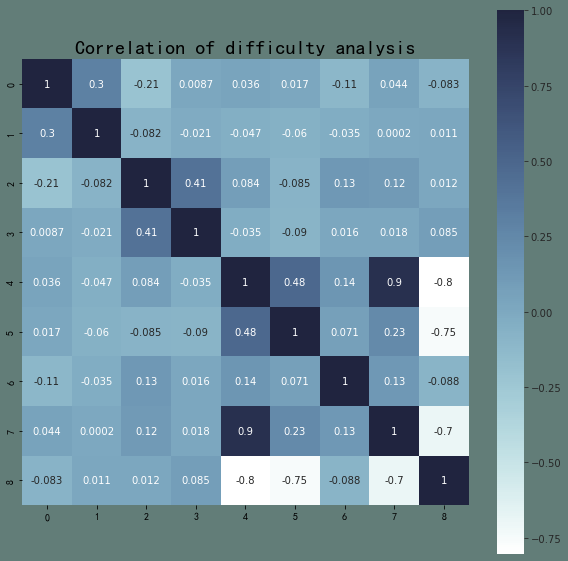
\includegraphics[height=12cm, width=12cm]{COR_dif.png}
	\caption{Correlations,0:difficult label,1:the number of repeated letters,2:the frequency of words,3:the number of vowels,4:hard mode,5:Zoom ratio,6:the frequency of wordle,7:date label}
\end{figure}
	
\begin{figure}[htbp]
	
	\centering
	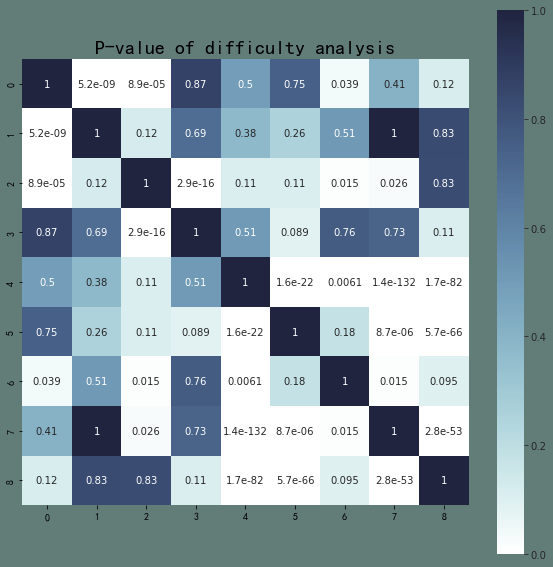
\includegraphics[height=12cm, width=12cm]{PER_dif.png}
	\caption{P-value,0:difficult label,1:the number of repeated letters,2:the frequency of words,3:the number of vowels,4:hard mode,5:Zoom ratio,6:the frequency of wordle,7:date label}
	
\end{figure}


\begin{figure}[htbp]
	
	\centering
	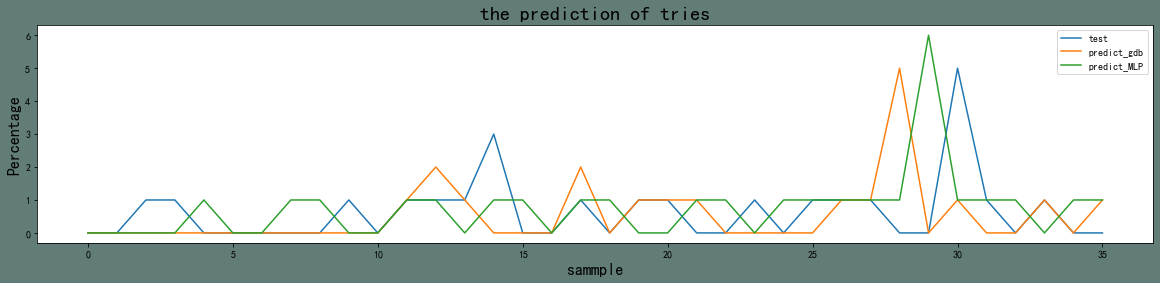
\includegraphics[height=4cm, width=16cm]{T1.png}
	\caption{The curve of the model}
	
\end{figure}

\newpage{}

\section{Model III : K-Means and KNN}
\subsection{Data Description}
In the data analysis stage, we read in the "tries" related columns from the raw data as a measure of difficulty and convert it into an $n * 7$ array .
We also compute the Pearson coefficient and its P-value of the tries,Results are shown in \textbf{Figure2,3}.

\subsection{Overview of the Model}
K-Means clustering is a method of vector quantization, originally from signal processing, that aims to partition n observations into k clusters in which each observation belongs to the cluster with the nearest mean, serving as a prototype of the cluster. This results in a partitioning of the data space into Voronoi cells. k-means clustering minimizes within-cluster variances, which would be the more difficult Weber problem: the mean optimizes squared errors, whereas only the geometric median minimizes Euclidean distances.

KNN is a type of classification where the function is only approximated locally and all computation is deferred until function evaluation. Since this algorithm relies on distance for classification, if the features represent different physical units or come in vastly different scales then normalizing the training data can improve its accuracy dramatically.
\subsection{The Establishment of Model III}
K-means clustering is a unsupervised machine learning algorithm used for clustering data points into groups based on their similarity.The requirement to partition the difficulty levels demands that we classify the data itself, and the data related to "tries" has a strong correlation. Therefore, K-means can solve this problem very well.

K-Nearest Neighbour,hereinafter referred to as ”KNN” , is a popular supervised machine learning algorithm used for classification and regression. In this model, we will focus on KNN as a classifier.KNN is a simple and effective algorithm for classifying data into multiple classes. The algorithm works by finding the K nearest data points to the target data point (the one we want to classify) in the feature space.Since we can obtain the classification of the original data through k-means, KNN can also be used as a classifier to predict the target point.

\subsection{The Solution of Model III and Question III}
We used K-means to divide all data points into 5 clusters and obtained the classification of each data point, which is shown in \textbf{Figure12,13}. Then we randomly split the dataset into training set and testing set in a 4:1 ratio. We used the data points in the training set as the original data, performed KNN classification on the testing set, obtained the test results and compared them with the testing set. We used accuracy\_score as the accuracy measurement standard, and the equation is as follows:
\begin{equation*}
	Accuracy\_Score = \frac{1}{n} \sum\limits_{i=1}^{n} 1|_{y_i = \hat{y}_i}
\end{equation*}

We were pleasantly surprised to find that its accuracy approached 100\%, which proved the accuracy of the classifier. Using difficulty\_score defined above we calculate the scores of the five clusters, name the clusters with five levels and list them in the table below.

\begin{center}
	

\begin{tabular}{c c}
\hline
Clusters&Difficulty Score\\
\hline
Very Hard & 23.6768\\
Hard & 17.1816\\
Normal & 13.2351\\
Easy & 10.6594\\
Very Easy & 8.4042\\
\hline
\end{tabular}

\vspace{0.3cm}
\textit{Table 3, categories of difficult.}
\end{center}



By using this classification algorithm and the data obtained from Model II, we categorized 'eerie' into \textbf{'Easy'} class.

\begin{figure}
	
	\centering
	
	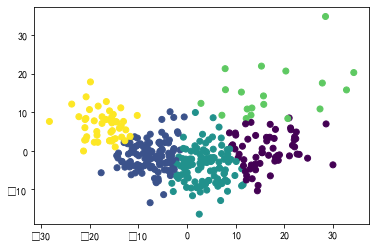
\includegraphics[height=9cm, width=13cm]{kmeans.png}
	\caption{kmeans}
\end{figure}
	
\begin{figure}[htbp]
	
	\centering
	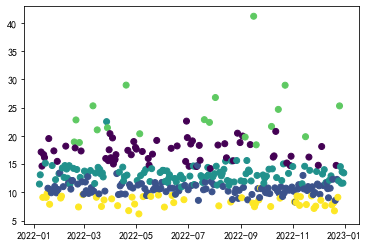
\includegraphics[height=9cm, width=13cm]{difficult.png}
	\caption{difficulty distribution}
	
\end{figure}

\newpage{}
\section{Sensitivity Test}
By conducting a previous correlation analysis, we obtained a sufficient number of non-relevant samples. We believe that it is normal for the model to have a fluctuation of around 15\% in prediction results when including some non-relevant samples or introducing some abnormal relevant samples. We used the model to train the data that contains mixed non-relevant and abnormal relevant samples, and obtained the results \textbf{Figure 14} with fluctuation around \textbf{5\%}. 

\begin{figure}[htbp]
	
	\centering
	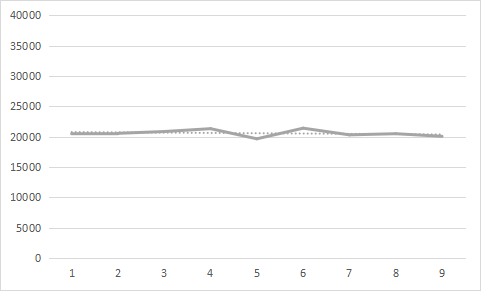
\includegraphics[height=6cm, width=13cm]{sensitive.png}
	\caption{sensitivity}
	
\end{figure}

As shown in the graph, the fluctuation in prediction results is small when adding non-relevant samples or introducing abnormal values, with an overall amplitude within 15\%.

Therefore, to a certain extent, we believe that our model is robust and practical. The model's prediction results will not change significantly due to an increase in non-relevant samples or some abnormal data.

\section{Evalution of Models}
\subsection{Strengths and Weakness}
\subsubsection{Strengths}
$\bullet$ Fitting good. For the current data, the prediction curve can have a good fitting degree and small upper and lower deviation.

$\bullet$ Apply widely on time scale. It can also be applied to future data without many code parameter revise.

\subsubsection{Weakness}
$\bullet$ The sample is too small. Our model lack train date which cause RMSE is not good enough.

$\bullet$ Too intuitive. Words all just intuitively select the attributes to develop and judge.
\subsection{Further Discussion}
$\bullet$ \textbf{For model improvement}, we may use voting and AdaBoost to improve our model.
 
$\bullet$ \textbf{For model expansion}, we used more than one crawler algorithm to obtain more data, and successfully obtained the word frequency data of Google search in recent years and the frequency statistics of words in published books in the past hundred years. (See the appendix for specific code)

However, it is obvious that due to the time limit of this project, we cannot obtain the real data about ten days before the forecast date (March 1). If we can continue to crawl the data, our model will be more accurate, so as to provide more realistic forecast results.

\section{Conclusion}
In this paper, our ultimate goal is to build models to predict the number of reported results and the distribution of reported results, as well as provide a model to classify words by difficulty. For these purposes, we have taken the following steps:
 \begin{enumerate}
	\item Firstly, we introduce an index 'Zoom Ratio' to measure the times of hard-mode numbers to reported-results numbers.
	\item Next, we build our \textbf{MLP(Multilayer Perceptron) Model} by using Python and Sklearn. For Grey Prediction and Polynomial Prediction for comparative uses, we build it on our code in appendix. 
	\item Then, we use MLP to predict the number of reported results on March 1, 2023.
	\item Also, we set up a GBDT and a MLP model and use both models to produce the prediction of the distribution of reported results.
	\item And then, we use K-means and KNN to classify words by distribution of tries to get word difficulty classification.
	\item Moreover, we test our model on sensitivity and point out their strengths and weakness.
	\item Finally, we use the models we build to write the letter to \textbf{\textit{New York Times}} puzzle editor.
 \end{enumerate}

 To conclude, the point of our models is to uso scientific means to instruct the 'Wordle' game for better performance.

 \section{Reference}

 We use Python Web Crawler to fetch frequency data of words from Google Books.(books.google.com)

\newpage
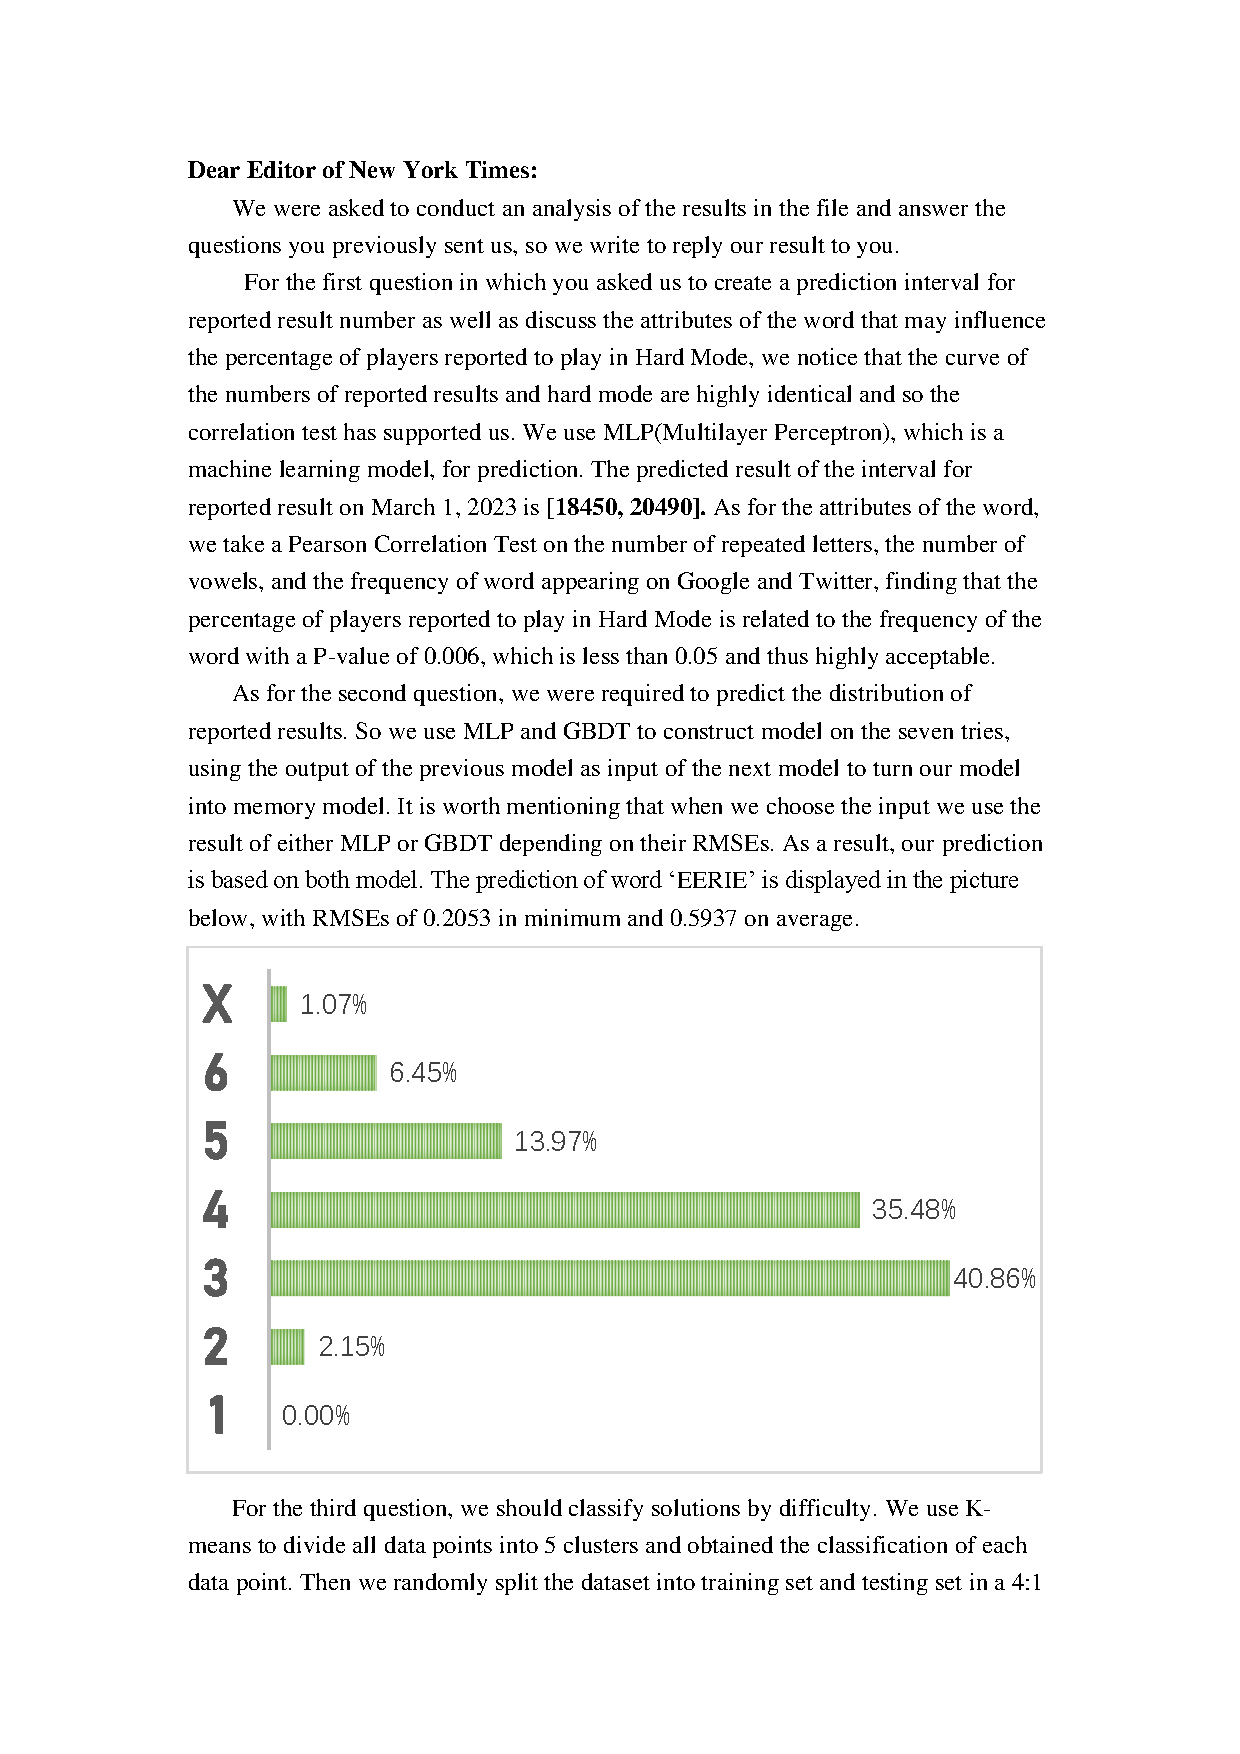
\includepdf[page={1,2}]{letter.pdf}

\newpage{}
\section{Appendix}
\vspace{2cm}
\begin{figure}[htbp]
	\centering
	\subfigure[]{
	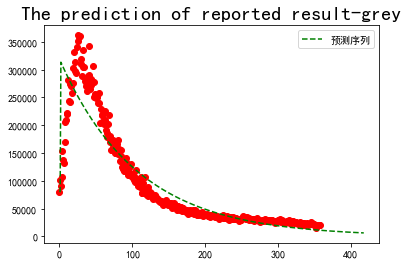
\includegraphics[width=7cm,height=3cm]{GREY_reported_result.png} \label{Fig.15(a)}
}
	\hspace{2mm}
	\subfigure[]{
	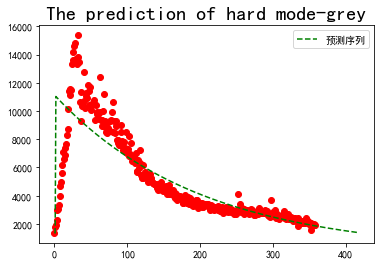
\includegraphics[width=7cm,height=3cm]{GREY_hard_mode.png} \label{Fig.15(b)}
}	
	\hspace{2mm}
	\subfigure[]{
		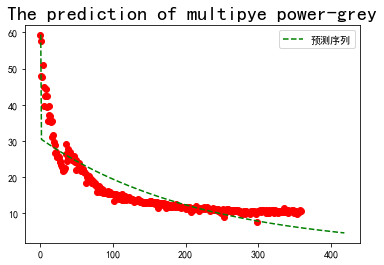
\includegraphics[width=7cm,height=3cm]{GREY_mul.png} \label{Fig.15(c)}
	}
	\caption{Three curves of Grey Prediction.}
\end {figure}

\begin{figure}[htbp]
	\centering
	\subfigure[]{
	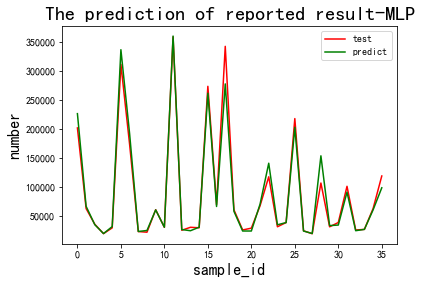
\includegraphics[width=6cm,height=3cm]{MLP_reported_result.png} \label{Fig.16(a)}
}
	\hspace{2mm}
	\subfigure[]{
	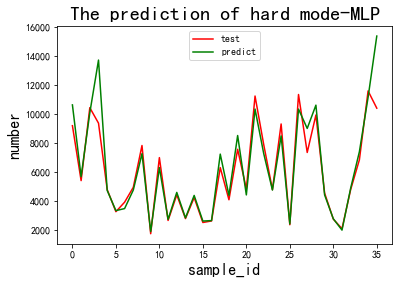
\includegraphics[width=6cm,height=3cm]{MLP_hard_mode.png} \label{Fig.16(b)}
}	
	\hspace{2mm}
	\subfigure[]{
		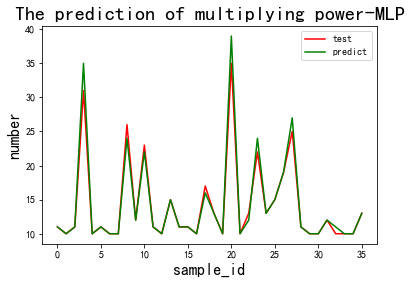
\includegraphics[width=6cm,height=3cm]{MLP_mul.png} \label{Fig.16(c)}
	}
	\caption{Three curves of Multilayer Perceptrons.}
\end {figure}

\newpage{}
\begin{figure}[htbp]
	\centering
	\subfigure[]{
	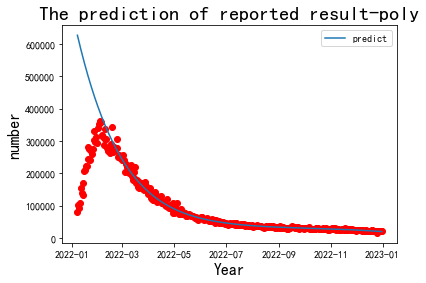
\includegraphics[width=6cm,height=3cm]{POLY_reported_result.png} \label{Fig.17(a)}
}
	\hspace{2mm}
	\subfigure[]{
	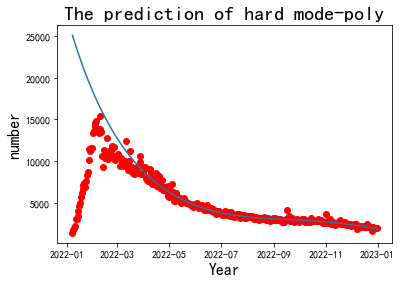
\includegraphics[width=6cm,height=3cm]{POLY_hard_mode.png} \label{Fig.17(b)}
}	
	\hspace{2mm}
	\subfigure[]{
		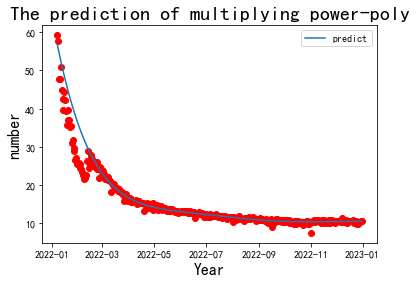
\includegraphics[width=6cm,height=3cm]{POLY_mul.png} \label{Fig.17(c)}
	}
	\caption{Three curves of Polynomial Prediction.}
\end {figure}

\begin{figure}[htbp]
	\centering
	\subfigure[]{
	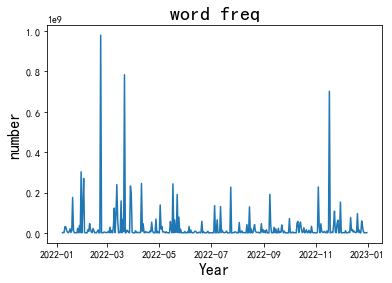
\includegraphics[height=3cm, width=6cm]{word_freq.png} \label{Fig.18(a)}
}
	\subfigure[]{
	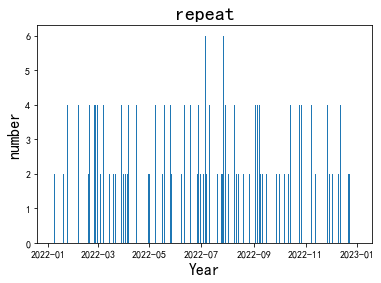
\includegraphics[height=3cm, width=6cm]{repeat.png} \label{Fig.18(b)}
}	
	\subfigure[]{
	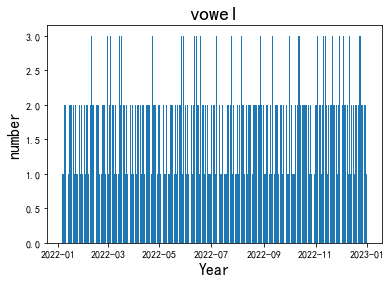
\includegraphics[height=3cm, width=6cm]{vowel.png} \label{Fig.18(c)}
}	
	\caption{curves of Other information.}
\end {figure}

\newpage{}
\begin{figure}[htbp]
	\centering
	\subfigure[]{
	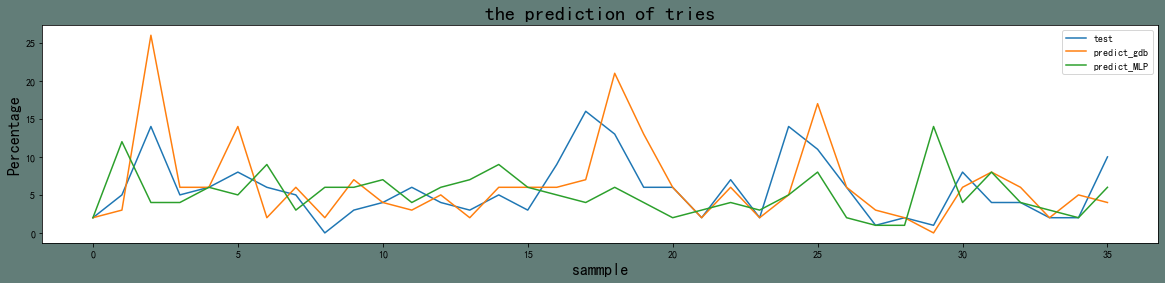
\includegraphics[width=12cm,height=3cm]{T2.png} \label{Fig.19(a)}
	}
	\hspace{2mm}
	\subfigure[]{
	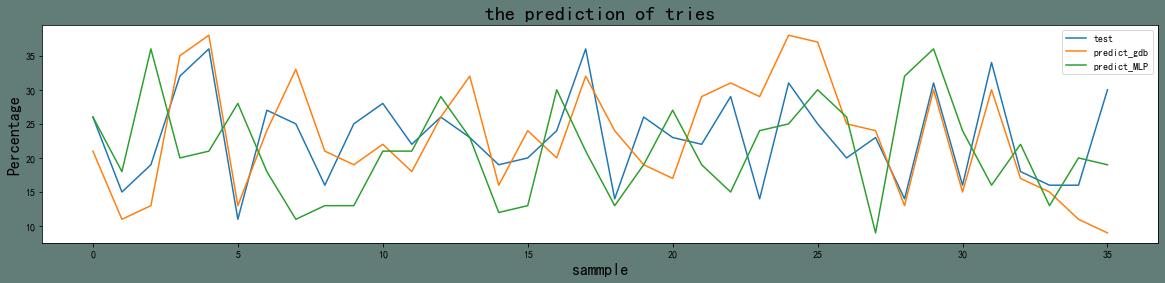
\includegraphics[width=12cm,height=3cm]{T3.png} \label{Fig.19(b)}
	}	
	\hspace{2mm}
	\subfigure[]{
		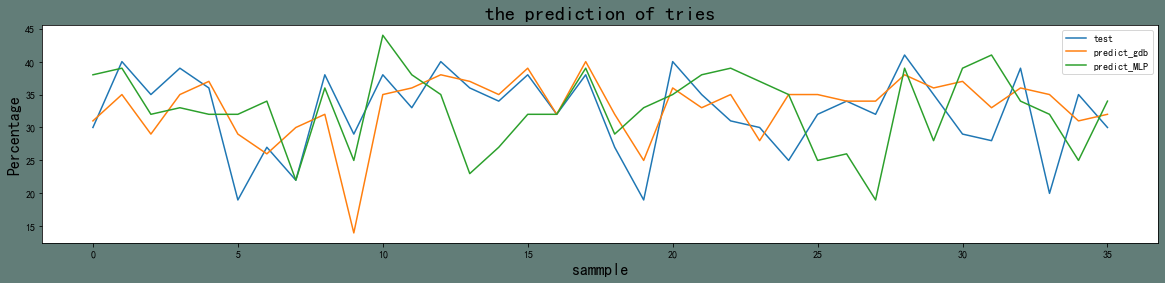
\includegraphics[width=12cm,height=3cm]{T4.png} \label{Fig.19(c)}
	}
	\hspace{2mm}
	\subfigure[]{
		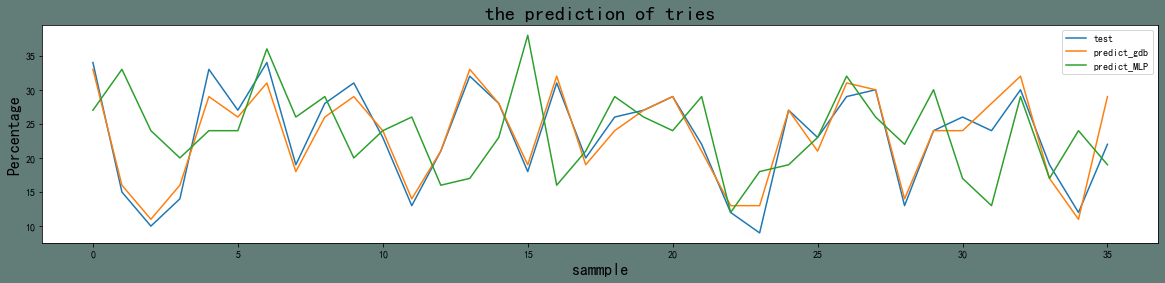
\includegraphics[width=12cm,height=3cm]{T5.png} \label{Fig.19(D)}
	}
	\hspace{2mm}
	\subfigure[]{
	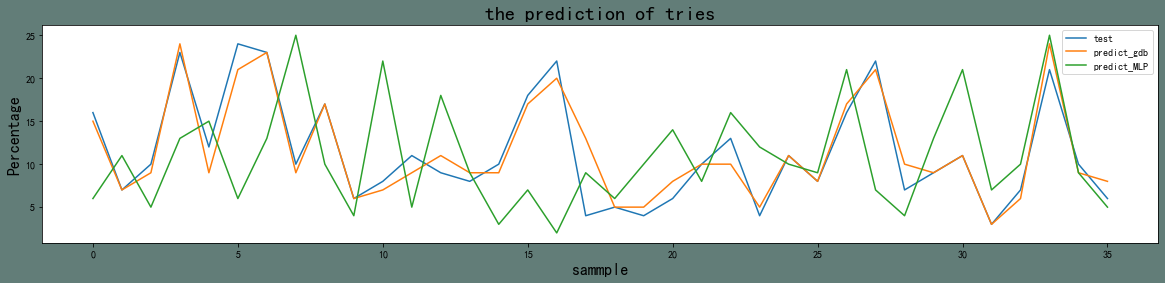
\includegraphics[width=12cm,height=3cm]{T6.png} \label{Fig.19(E)}
	}	
	\hspace{2mm}
	\subfigure[]{
		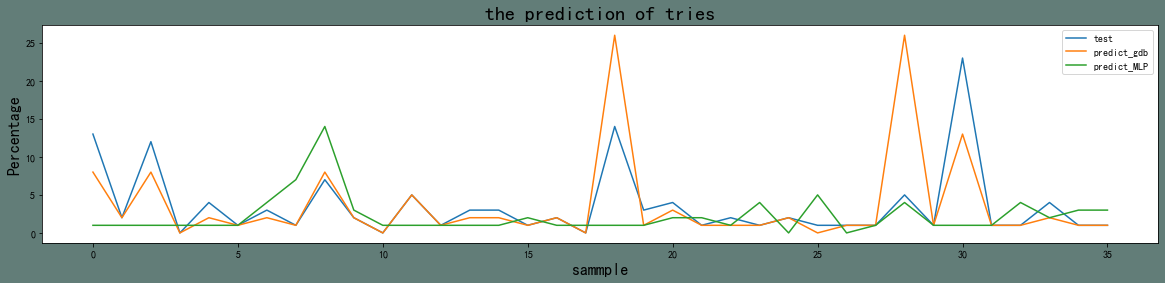
\includegraphics[width=12cm,height=3cm]{T7.png} \label{Fig.19(F)}
	}
	\caption{Three curves of Polynomial Prediction.}
\end {figure}

\newpage{}
%%%%%%%%%%%%%%%%%%%%%%%%%%%%%%
\end{document}
\end
